%----------------------------------------------------------------------------------------
% PACKAGES AND DOCUMENT CONFIGURATIONS
%----------------------------------------------------------------------------------------

  \documentclass[12pt]{article}

  \usepackage{hyperref}
  \usepackage{fancyhdr} % Required for custom headers
  \usepackage{lastpage} % Required to determine the last page for the footer
  \usepackage{extramarks} % Required for headers and footers
  \usepackage[usenames,dvipsnames]{color} % Required for custom colors
  \usepackage{graphicx} % Required to insert images
  \usepackage{listings} % Required for insertion of code
  \usepackage{courier} % Required for the courier font
  \usepackage{lipsum} % Used for inserting dummy 'Lorem ipsum' text into the template
  \usepackage{wrapfig}
  \usepackage{color}
  \usepackage{lscape}

  \setlength\parindent{0pt} % Removes all indentation from paragraphs
  \renewcommand{\labelenumi}{\alph{enumi}.} % Make numbering in the itemize environment by letter rather than number (e.g. section 6)
  \lstset{basicstyle=\ttfamily\footnotesize,breaklines=true}

  % Margins
  \topmargin=-0.4in
  \evensidemargin=0.2in
  \oddsidemargin=-0.2in
  \textwidth=7.0in
  \textheight=9.0in
  % \headsep=0.25in

  % \linespread{1.1} % Line spacing

  \definecolor{dkgreen}{rgb}{0,0.6,0}
  \definecolor{gray}{rgb}{0.5,0.5,0.5}
  \definecolor{mauve}{rgb}{0.58,0,0.82}
  \definecolor{greyish}{rgb}{0.96,0.96,0.96}

  \lstset{
    backgroundcolor=\color{greyish},   % choose the background color; you must add \usepackage{color} or \usepackage{xcolor}
    frame=tblr,
    numbers=left,                       % where to put the line-numbers; possible values are (none, left, right)
    numbersep=5pt,                   % how far the line-numbers are from the code
    numberstyle=\tiny\color{mygray}, % the style that is used for the line-numbers
    language=Ruby,
    aboveskip=3mm,
    belowskip=3mm,
    showstringspaces=false,
    columns=flexible,
    basicstyle={\footnotesize\ttfamily},
    numbers=none,
    numberstyle=\tiny\color{gray},
    keywordstyle=\color{blue},
    commentstyle=\color{dkgreen},
    stringstyle=\color{mauve},
    breaklines=true,
    breakatwhitespace=true
    tabsize=1
  }

  \begin{document}
  \begin{titlepage}

%----------------------------------------------------------------------------------------
% TITLE PAGE INFORMATION
%----------------------------------------------------------------------------------------
 \newcommand{\HRule}{\rule{\linewidth}{0.5mm}} % Defines a new command for the horizontal lines, change thickness here
  \begin{center} % Center everything on the page

  %----------------------------------------------------------------------------------------
  % HEADING SECTIONS
  %----------------------------------------------------------------------------------------
  \textsc{\large Faculty of Computers, Informatics and Microelectronics}\\[0.5cm]
  \textsc{\large Technical University of Moldova}\\[1.2cm] % Name of your university/college
  \vspace{35 mm}
  \textsc{\Large PAD}\\[0.5cm] % Major heading such as course name
  %\textsc{\large Laboratory work \#1-3}\\[0.5cm] % Minor heading such as course title
  \textsc{\large Laboratory work \# 3}\\[0.5cm] % Minor heading such as course title

  %----------------------------------------------------------------------------------------
  % TITLE SECTION
  %----------------------------------------------------------------------------------------
  \vspace{10 mm}
  \HRule \\[0.4cm]
  { \large \bfseries   Study of HTTP protocol used in distributed systemns  }\\[0.4cm] % Title of your document
  \HRule \\[1.5cm]

  %----------------------------------------------------------------------------------------
  % AUTHOR SECTION
  %----------------------------------------------------------------------------------------
      \vspace{30mm}

      \begin{minipage}{0.4\textwidth}
      \begin{flushleft} \large
      \emph{Authors:}\\
      \textbf{Petru \textsc{Negrei}} \\
      Victor \textsc{Vasilica}
      \end{flushleft}
      \end{minipage}
      ~
      \begin{minipage}{0.4\textwidth}
      \begin{flushright} \large
      \emph{Supervisor:} \\
      D. \textsc{Ciorba} % Supervisor's Name
      \end{flushright}
      \end{minipage}\\[4cm]

      \vspace{5 mm}
      % If you don't want a supervisor, uncomment the two lines below and remove the section above
      %\Large \emph{Author:}\\
      %John \textsc{Smith}\\[3cm] % Your name

      %----------------------------------------------------------------------------------------
      % DATE SECTION
      %----------------------------------------------------------------------------------------

      {\large November 2014}\\[3cm] % Date, change the \today to a set date if you want to be precise

      %----------------------------------------------------------------------------------------
      % LOGO SECTION
      %----------------------------------------------------------------------------------------

      %\includegraphics{Logo}\\[1cm] % Include a department/university logo - this will require the graphicx package

      %----------------------------------------------------------------------------------------

      \vfill % Fill the rest of the page with whitespace
      \end{center}
      \end{titlepage}

      % \newpage
      % \tableofcontents
      % \newpage

%----------------------------------------------------------------------------------------
% Introduction
%----------------------------------------------------------------------------------------

  \section{Introduction}

  \subsection{Topic}

  Study of HTTP protocol used in distributed systemns. 
  Implementation of connection between client and server using HTTP methods.

  \subsection{Objective}

  Implementation of the thread safe system of processing of data.

  \subsection{Generic requirements}

  \subsubsection{Report}

  Report will contain a short description of work done, and will present necesary information
  about tools, algorithms used or studied.

%----------------------------------------------------------------------------------------
% Implementation
%----------------------------------------------------------------------------------------
  
  \section{Structure}

    Below you can see the structure of the application, there are represented the classes used 
    and their variables and methods. The main are client and server which the helper class 
    \textit{Http Handler} that server the purpose of sending the http requests to the \textit{Main Server.} \\

    The client will be responsible for sending \textit{GET} request to the \textit{Main Server}, then the 
    \textit{Main Server} will find the node with max connections and return the information to the \textit{Client}
    Then the \textit{Client} will establish a TCP connection necessary node. After it receive all necesary data, this 
    data will be analyzed and shown to the user. \\ 

    In order to allow multiple requests from server nodes and client, each connection will be handled in different
    thread and in a safe way.

    \begin{minipage}[b]{1.0\linewidth}
      \begin{center}
        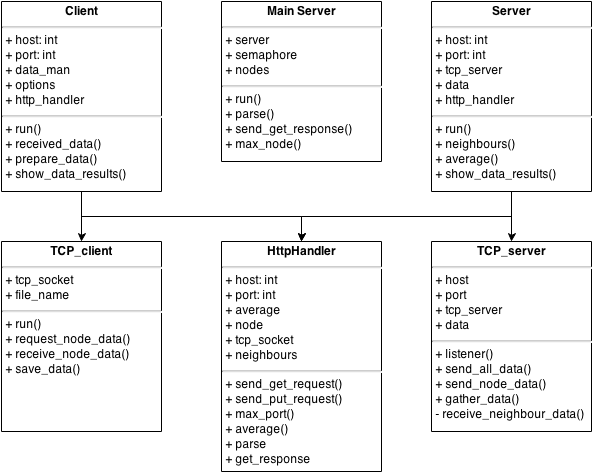
\includegraphics[width=0.8\textwidth]{diagram}
         \\ Fig. 1 Class diagram
      \end{center}
    \end{minipage}
    
  \section{Implementation}

    \subsection{Stored data}

    Like in the previous laboratory work all information of servers is stored in one single \textit{json} file (\textit{data.json}) 
    in order to reduce redundancy in real project each server will have separate file that will contain its specific data. 
    
    \begin{lstlisting}
    {
      "10000": {
        "neigthbours": [10001],
        "employers":[ ... ]
      },
      # ... 
    }
    \end{lstlisting}

    \begin{lstlisting}
    # ...
        "employers":[
            {"firstName":"John",     "lastName":"Doe",       "salary": 150, "department": "Marketing"},
            ...
            {"firstName":"Alex",     "lastName":"Carturari", "salary": 478, "department": "Testing"}
         ]
    # ...
    \end{lstlisting}

    \subsection{Client Side}

    The client part of the application is composed of four main file that together provide functionality
    necesary to assure the request to server, receive, save, parse and show the response in form of the
    list of emplyoers from server with the maximum nodes and its neighbours.

    \subsubsection{HTTP handler}

    We don't use the UDP helper like in the previous laboratory work, instead we send the \textit{GET} request
    to the \textit{Main Server} and receive the response that will contain the port and average of the node with
    maximum connections.

    \begin{itemize}
      \renewcommand{\labelitemi}{$\circ$}
      \item  \textit{initialize} - initialize all necesary variables and a TCP socket.
      \item \textit{send\_get\_request} - send \textit{GET} request and receives the response from \textit{Main Server}.
      \item \textit{send\_put\_request} - send \textit{PUT} request in the case of server node.
      \item \textit{max\_port} - returns the node with max connections.
      \item \textit{average} - computes the total average of all nodes.
    \end{itemize}

    \begin{lstlisting}
     class HttpHandler

        attr_accessor :host, :node, :tcp_socket, :port, :neighbors, :average

        def initialize host, port, neighbors=0, average=0
          @host = host
          @neighbors = neighbors
          @average = average
          @node = {}
          @port = port
          @tcp_socket = TCPSocket.new(host, 8000)
        end

        def send_get_request
          tcp_socket.puts "GET / HTTP/1.0\r\n\r\n"
          parse get_response
          tcp_socket.close
        end

        def send_put_request
          response = "#{port}:#{neighbors}:#{@average}"
          header = [ "PUT / HTTP/1.0",
                     "HOST: #{host}",
                     "Content-Type: text/plain",
                     "Content-Length: #{response.bytesize}",
                     "Connection: Keep-Alive" ].join "\r\n"

          tcp_socket.puts header + "\r\n\r\n" + response
          p "sent put request"
          tcp_socket.close
        end

        def max_port
          @node["port"]
        end

        def average
          @node["average"]
        end

        private

        def parse response
          @node = JSON.parse response
        end 

        def get_response
         response = ''
          while line = tcp_socket.recv(1024)
            response += line
            line =~ /%--%/  ? break : response += line
          end
          headers,body = response.split(/\r\n\r\n/)
          body.gsub "%--%", ""
        end

      end
    \end{lstlisting}

    \subsubsection{TCP protocol Data manipulation}

    It were implemented in the previous laboratory work.
  
    \subsection{Main Server}

    The most important function of the main server is to receive different request, and 
    depending on type and parameters of request to perform certain actions.  \\

    The \textit{run} function is the function that receives requests from nodes or
    client in a thread safe way and depending of the type of request it acess different 
    methods. 

    \begin{lstlisting}
    # ...
      def run
        loop do
         Thread.start(server.accept) do |client|
            @semaphore.synchronize do
              request = client.gets
              if request =~ /^GET.*/
                send_get_response(client)
              else
                request += client.read
                @nodes << request
              end
              client.close
            end
          end
        end
      end
    # ... 
    \end{lstlisting}
        
    \subsubsection{Main}

    The main class \textit{Client} contains all methods that are necesary to start and perform necesary
    work, it also has UDP and TCP functionality by using the  \textit{classes} with the same name.
    Below there is a short description of methods that it has, for the implementation you can see the full code.

    \begin{itemize}
      \renewcommand{\labelitemi}{$\circ$}
      \item In the \textit{contructor} we save provided options and setup http handler.
      \item  \textit{receive\_data} - we setup a tcp server, send requests to servers and save response to a file.
      \item \textit{prepare\_data} - read the json file and initiate the data manipulation class.
      \item \textit{show\_data\_results} - show data received from server, based on option from console.
    \end{itemize}

    \begin{lstlisting}
    class Client
      # ... 
      def initialize options
        @options = options
        @http_client = HttpHandler.new HOST, 8000
      end

      def run
        # ...
      end

      private

        def receive_data
          tcp_client = TcpClient.new(HOST, FILE_NAME, http_client.max_port)
          tcp_client.run
        end

        def prepare_data
          data = read_json_file
          @data_man = DataManipulation.new(data, http_client.average)
        end

        def show_data_results
          case options[:show]
          when "default"   then data_man.show_all
          when "filtered"   then data_man.show_filtered
          else
            puts "Invalid option"
          end
        end

        def read_json_file
          JSON.parse File.read(FILE_NAME)
        end

    end

    # input arguments from terminal
    options = {}
    options[:show] = "default"
    OptionParser.new do |opts|
      opts.banner =  "Usage: ruby client.rb [options]\n\n"
      opts.on("-s", "--show [SHOW]", "show data by method") do |s|
        options[:show] = s || "default"
      end
    end.parse!
    \end{lstlisting}

    One of its most important methods is `run` method, here we first send
    get request to the \textit{Main Server} and then we establish a tcp connection with the node
    with maximum neighboars, receiving necesary information from it, parse it and show it
    in the console.

    \begin{lstlisting}
    # ...
      def run
        http_client.send_get_request
        receive_data
        prepare_data
        show_data_results
      end
      # ...
    \end{lstlisting}

    The client actions are started with the following line, it receive the actions that need to be applied on the data.

    \begin{lstlisting}
    Client.new(options).run
    \end{lstlisting}

    \subsection{Servers}

    The \textit{Main server} part was done by Vasilica Victor but a part of functionality of thread safe implementation was done working together, 
    (pair programming) in order to assure the integrity of the data.

    \section{Conclusion}

    In this laboratory work we built a distributed system that different http requests to send information from nodes to main server
    and from \textit{main server} to \textit{client}, each request doing its own predefined task.

    We build a helper class that handles all required requests \textit{GET} and \textit{PUT}, and receives the responses from the \textit{Main Server}.
    Depending on the request \textit{Main Server} will perform different action, in the \textit{GET} case it will return the information about 
    node with maximum connection, when \textit{PUT} it will add the information in an array.

    Thus we learned how to build a small distributed system with a collection of objects using different http requests. \\

    \textbf{Link to Repository: } \url{https://gitlab.ati.utm.md/petru.negrei/lab3/tree/wip/petru}


   \section{References}

   \begin{itemize}
      \item Ruby Socket \url{http://www.ruby-doc.org/stdlib-1.9.3/libdoc/socket/rdoc/Socket.html}
      \item Ruby TCP  Socket \url{http://www.ruby-doc.org/stdlib-1.9.3/libdoc/socket/rdoc/TCPSocket.html}
      \item Ruby Mutex \url{http://wwwi.ruby-doc.org/core-2.1.4/Mutex.html}
      \item Ruby JSON \url{http://www.ruby-doc.org/stdlib-2.0.0/libdoc/json/rdoc/JSON.html}
      \item Ruby OptionParser \url{http://ruby-doc.org/stdlib-2.1.0/libdoc/optparse/rdoc/OptionParser.html}
   \end{itemize}


\end{document}

